\documentclass[aspectratio=169]{beamer} % Imposta aspect ratio 16:9 per layout moderno
\usepackage[utf8]{inputenc}
\usepackage[T1]{fontenc}
\usepackage{lmodern}
\usepackage{amsmath}
\usepackage{amssymb}
\usepackage{graphicx}
\usepackage{booktabs} % Per tabelle più pulite
\usepackage{silence} % Silenzia warning inutili che intasano il log
\WarningFilter{beamerthememadrid}{You have requested}

\disablemag

% --- SCELTA DEL TEMA E PERSONALIZZAZIONE ---
\usetheme{Madrid}
\usecolortheme{default}
\useinnertheme{circles} % Pallini più eleganti
\usefonttheme{professionalfonts} % Migliore resa delle formule matematiche

% --- FIX PER IL FOOTER (BARRA IN BASSO) ---
% Riduce la dimensione del font nella barra inferiore per evitare testi tagliati
\setbeamerfont{author in head/foot}{size=\fontsize{6}{7}\selectfont}
\setbeamerfont{title in head/foot}{size=\fontsize{6}{7}\selectfont}
\setbeamerfont{date in head/foot}{size=\fontsize{5}{6}\selectfont}

% --- INFORMAZIONI DI COPERTINA ---
% Tra parentesi quadre [] metto il testo corto per la barra sotto
% Tra graffe {} metto il testo completo per la slide
\title[Ottimizzazione Reattore Sottocritico]{Ottimizzazione dei parametri di operatività di un reattore sottocritico}
\author[R. Bossi]{Riccardo Bossi \\ \small Mat: 881923}
\institute[PoliMi \& Bicocca]{Università degli Studi di Milano-Bicocca \\ Politecnico di Milano}

% Per gestire correttamente Relatore e Correlatrice
\author[R. Bossi]{
  Riccardo Bossi \\ \medskip
  {\small Relatore: Prof. Antonio Cammi} \\
  {\small Correlatrice: Prof.ssa Monica Sisti}
}
\date{\today}

\begin{document}

% --- SLIDE TITOLO ---
\begin{frame}
  \titlepage
\end{frame}
% --- SLIDE DI CONTESTO (Nuova) ---
\begin{frame}{Il Sistema Sottocritico: Concetti Chiave}
    Un reattore sottocritico ($k_{eff} < 1$) non può mantenere una reazione a catena autosostenuta. La popolazione neutronica e la potenza termica dipendono strettamente da una \textbf{sorgente esterna} di neutroni.

    \vspace{0.4cm}
    \begin{itemize}
        \item \textbf{Relazione Potenza-Sorgente:} In regime stazionario, la potenza $P$ è direttamente proporzionale all'intensità della sorgente $S$.
        \item \textbf{Controllo dell'Operatività:} Modificando l'intensità della sorgente (es. corrente del fascio dell'acceleratore), si modifica linearmente la potenza del reattore.
        \item Le variazioni di potenza causano variazioni termiche che, tramite i \textbf{feedback di reattività}, modificano il valore del $k_{eff}$ stesso.
    \end{itemize}

    \vspace{0.3cm}
    \begin{exampleblock}{Domanda di Ricerca}
        In che modo le operazioni sulla sorgente (che determinano il passaggio tra gli stati di operatività) influenzano il $k_{eff}$ e come possiamo ottimizzare questo legame garantendo la sicurezza?
    \end{exampleblock}
\end{frame}

\begin{frame}{Stati di Operatività del Reattore}
    Supponendo di avere un reattore sottocritico, potremmo modellare come segue i suoi stati di funzionamento:
    
    \vspace{0.3cm}
    \begin{itemize}
        \item \textbf{Cold Zero Power (CZP):} Condizione di equilibrio termico globale. Combustibile e moderatore si trovano a $300 \text{ K}$. Il reattore risulta spento.
        \onslide<2->{
        \item \textbf{Hot Zero Power (HZP):} Assenza di produzione di potenza termica macroscopica. L'equilibrio termico garantisce $T_{fuel} \sim T_{mod}$, con l'acqua che raggiunge la temperatura operativa del sistema: $350 \text{ K}$. Questa situazione corrisponde alla fase di accensione.
        }
        \onslide<3->{
        \item \textbf{Hot Full Power (HFP):} Estrazione di potenza nominale. Si stabilisce un gradiente termico dinamico: le barre di combustibile si scaldano fino a $600 \text{ K}$, cedendo calore all'acqua ($350 \text{ K}$) impiegata nel ciclo termodinamico. il reattore è in regime di operatività.
        }
    \end{itemize}
\end{frame}

\begin{frame}{Scopo del mio lavoro di tesi}

Muovendosi da HFP a CZP la temperatura si abbassa, ma a causa dei feedback, il $k_{eff}$ si alza:

    \begin{alertblock}{Ottimizzazione delle Prestazioni}
        Sviluppare una metodologia sistematica per individuare le condizioni operative ottime di un reattore sottocritico ($k_{eff} < 1$), massimizzando l'autovalore operativo $k_{HFP}$ nel rigoroso rispetto dei vincoli di sicurezza per ogni transitorio termico ($k_{CZP} < 1$).
    \end{alertblock}
    
    \vspace{0.4cm}
    \onslide<2->{
    \begin{block}{Indipendenza Parametrica del Modello}
        La routine di ottimizzazione è agnostica rispetto alla configurazione di base. Non vengono fatte ipotesi a priori su geometria, raggi del combustibile o materiali del target. L'intero set di parametri è gestito in modo dinamico tramite un file di configurazione \texttt{.txt}.
    \end{block}
    }
\end{frame}


\begin{frame}{Layout Geometrico del Reattore}
    \begin{figure}
        \centering
        % Usiamo due minipage speculari per centrare le immagini nei due "mezzi" della slide
        \begin{minipage}{0.48\textwidth}
            \centering
            
\includegraphics[width=0.85\linewidth]{reactor_xy.png}
            \caption{Sezione piano XY.}
        \end{minipage}
        \begin{minipage}{0.48\textwidth}
            \centering
            
\includegraphics[width=0.65\linewidth]{reactor_xz.png} % Larghezza ridotta per compensare l'altezza
            \caption{Sezione piano XZ.}
        \end{minipage}
    \end{figure}
\end{frame}

\begin{frame}{Progetto SYNERGY}
    \begin{block}{Sistema Synchrotron-driven Neutron source}
        Infrastruttura progettata per colmare il gap di flusso tra le grandi sorgenti a spallazione (\sim $10^{16}$ n/$cm^2$ s) e le macchine compatte (CANS: \sim $10^{10}$ n/$cm^2$ s). Attualmente in fase di studio.
    \end{block}
    
    \begin{itemize}
        \item Produzione di fotoni $\gamma$ mediante magneti curvanti in anelli di accumulazione ad alta energia.
        \item Estrazione tangenziale del fascio su target esterni per la generazione di neutroni via reazione fotonucleare.
    \end{itemize}
    
    \begin{columns}[c]
        \begin{column}{0.45\textwidth}
                \footnotesize
                \textbf Figura3: Layout dell'anello di accumulazione e delle beamline di estrazione del fascio fotonico.
                \label{fig:synergy_ring}
            
        \end{column}
        
        \begin{column}{0.55\textwidth}
    
            \centering
            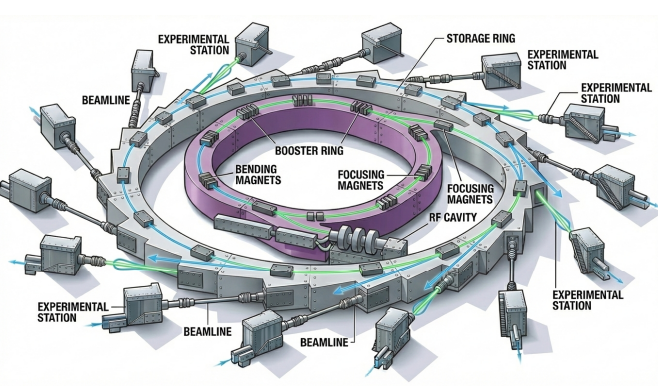
\includegraphics[width=0.8\textwidth]{Sincrotrone_anello.png}
        
        \end{column}
    \end{columns}
\end{frame}

\begin{frame}{Spettro di Funzionamento e Intensità della Sorgente}
    \begin{columns}
        \begin{column}{0.5\textwidth}
            \begin{itemize}
                \item \textbf{Spettro energetico:} Spettro continuo tra $1$ e $37 \text{ MeV}$, che copre la regione della \textit{Giant Dipole Resonance} (GDR) dei bersagli. In questa regione l'Uranio si eccita assorbendo un fotone, segue poi diseccitazione con emissione di neutrone/i. Domina il processo $(\gamma,n)$ che raggiunge un picco a 14 MeV con 500 mb.  
                \item \textbf{Intensità primaria:} Rate fotonico di $S_\gamma = 2.02 \times 10^{17} \gamma/\text{s}$ per singola beamline.
                \item \textbf{Potenza di generazione:} $\sim 200 \text{ kW}$ per fascio fotonico.
            \end{itemize}
        \end{column}
        
        \begin{column}{0.5\textwidth}
            \begin{figure}
                \centering
                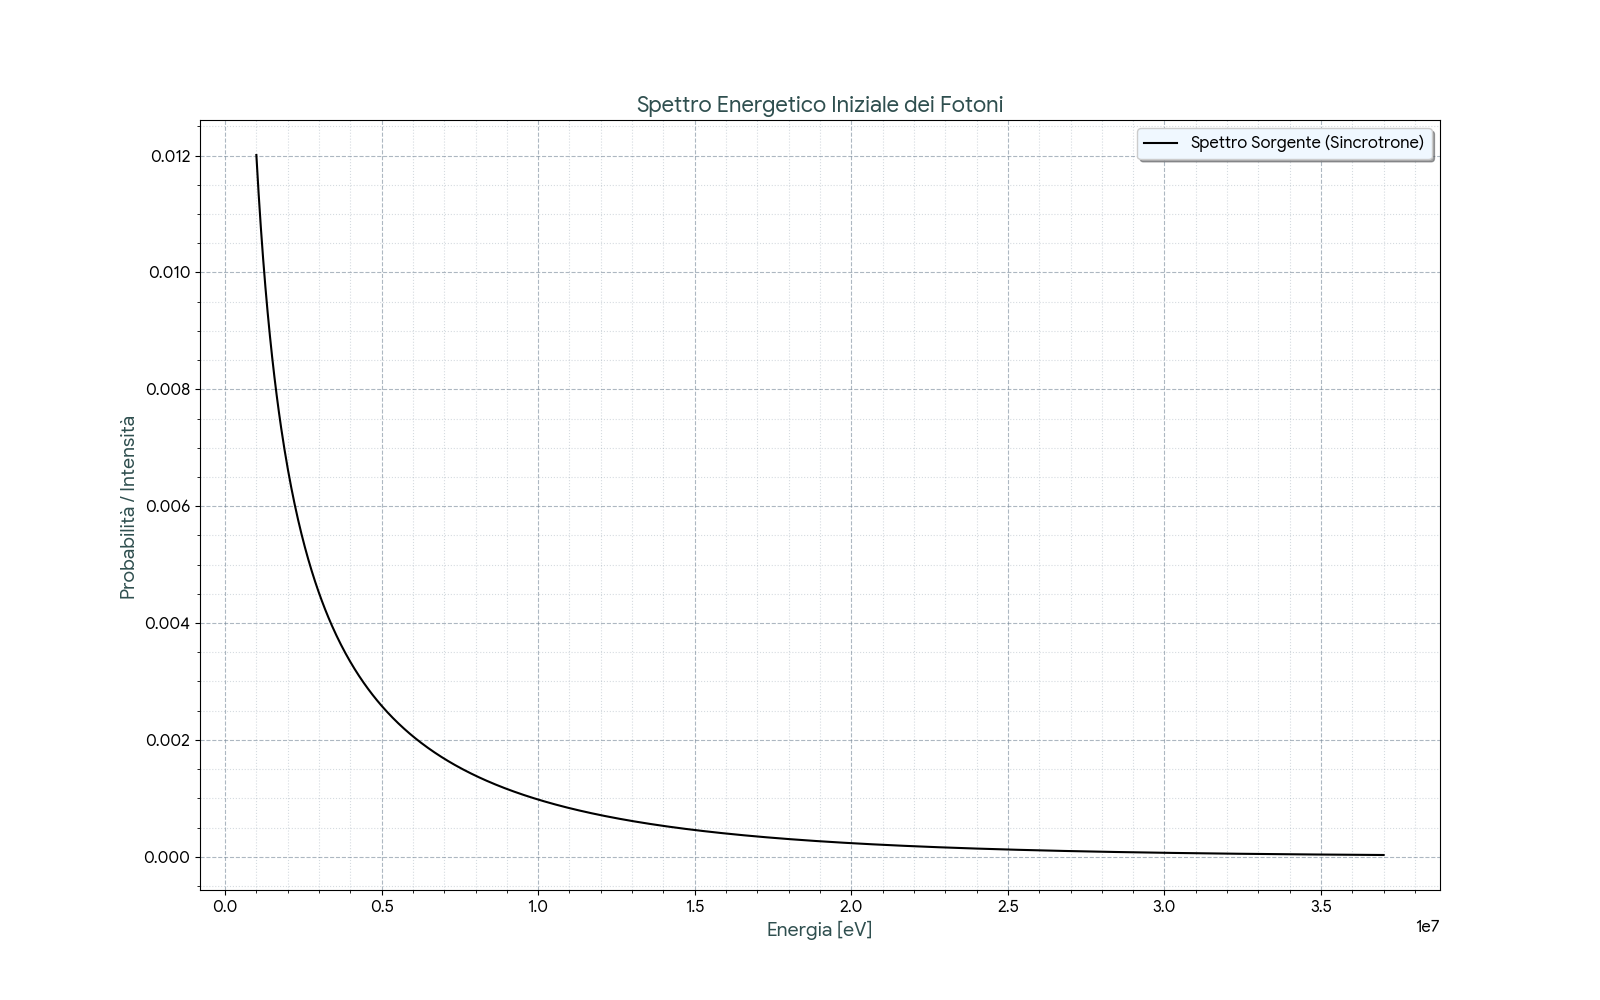
\includegraphics[width=\linewidth]{syncro_spectrum.png}
                \caption{Distribuzione energetica della radiazione di sincrotrone incidente ($1-37 \text{ MeV}$).}
                \label{fig:spectrum}
            \end{figure}
        \end{column}
    \end{columns}
\end{frame}

\begin{frame}{Dinamica del Difetto di Reattività}
    Perché la reattività varia durante i transitori?
    
    \vspace{0.3cm}
    \begin{itemize}
        \item \textbf{Effetto Densità Moderatore:} L'aumento di temperatura riduce la densità dell'acqua, degradando il potere rallentante e alterando il bilancio tra fughe neutroniche e catture parassite.
        \onslide<2->{
        \item \textbf{Effetto Doppler:} L'incremento dell'agitazione termica dei nuclei di $^{238}\text{U}$ nel reticolo cristallino del $\text{UO}_2$ induce il \textit{broadening} delle sezioni d'urto di cattura risonante.
        }
    \end{itemize}
    
    \vspace{0.4cm}
    \onslide<3->{
    \begin{alertblock}{Variazione di Reattività Globale}
        Per una transizione termodinamica tra due stati, il $\Delta\rho$ è formalizzato come:
        \begin{equation*}
            \Delta\rho = \rho_2 - \rho_1 = \frac{k_2 - 1}{k_2} - \frac{k_1 - 1}{k_1} = \frac{k_2 - k_1}{k_1 \cdot k_2}
        \end{equation*}
    \end{alertblock}
    }
\end{frame}

\begin{frame}{Superficie di Moltiplicazione Termodinamica}
    \begin{columns}[c]
        % Colonna Sinistra: Immagine
        \begin{column}{0.45\textwidth}
            \centering
            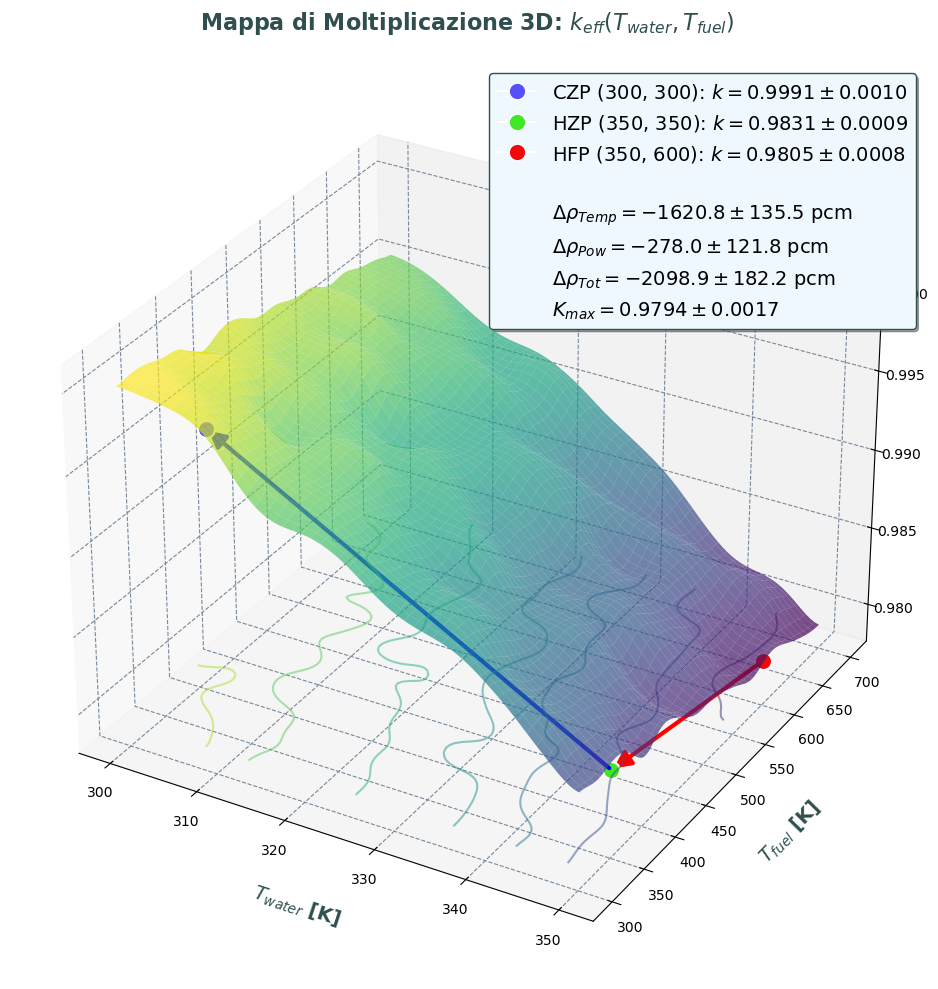
\includegraphics[width=\textwidth]{superficie.png}
        \end{column}
        
        % Colonna Destra: Didascalia (Testo semplice)
        \begin{column}{0.32\textwidth}
        
            \footnotesize
            \textbf{Figura 4:} Mappa 3D dell'autovalore $k_{eff}$ in funzione delle temperature di moderatore ($T_{water}$) e combustibile ($T_{fuel}$) nei transitori HFP $\rightarrow$ CZP.
            
            \vspace{0.4cm}
            Il grafico evidenzia il forte incremento di reattività indotto dall'espansione termica del moderatore e dall'allargamento Doppler delle risonanze dell'U-238.
            
        \end{column}
    \end{columns}
\end{frame}

\begin{frame}{Valutazione del $k_{max}$ e Analisi Parametrica}
    Il margine massimo di reattività impostabile a freddo è vincolato dal bilancio dei coefficienti di reattività integrali:
    
    \begin{equation*}
        k_{max} = 1 - \Delta\rho_{doppler} - \Delta\rho_{water} - \Delta\rho_{ignoranza} - \dots
    \end{equation*}

\begin{block}{Margine di sicurezza}
Importante notare che è stato inserito un margine di sicurezza pari a $200$ $pcm$ inerente l'ignoranza dei dati sulle librerie in uso.
\end{block}

    
    \vspace{0.5cm}
    \onslide<2->{
    \begin{block}{Impatto della Pressione Operativa}
        Diverse simulazioni a reticolo (Pitch) e Pressione variabili hanno dimostrato che \textbf{l'effetto della pressione è del second'ordine}. Di conseguenza, la suite di simulazioni di design è stata consolidata alla pressione atmosferica ($1 \text{ atm}$).
    \end{block}
    }
\end{frame}

\begin{frame}{Dipendenza non-lineare di $k_{max}$ dal Pitch}
    \begin{figure}
        \centering
        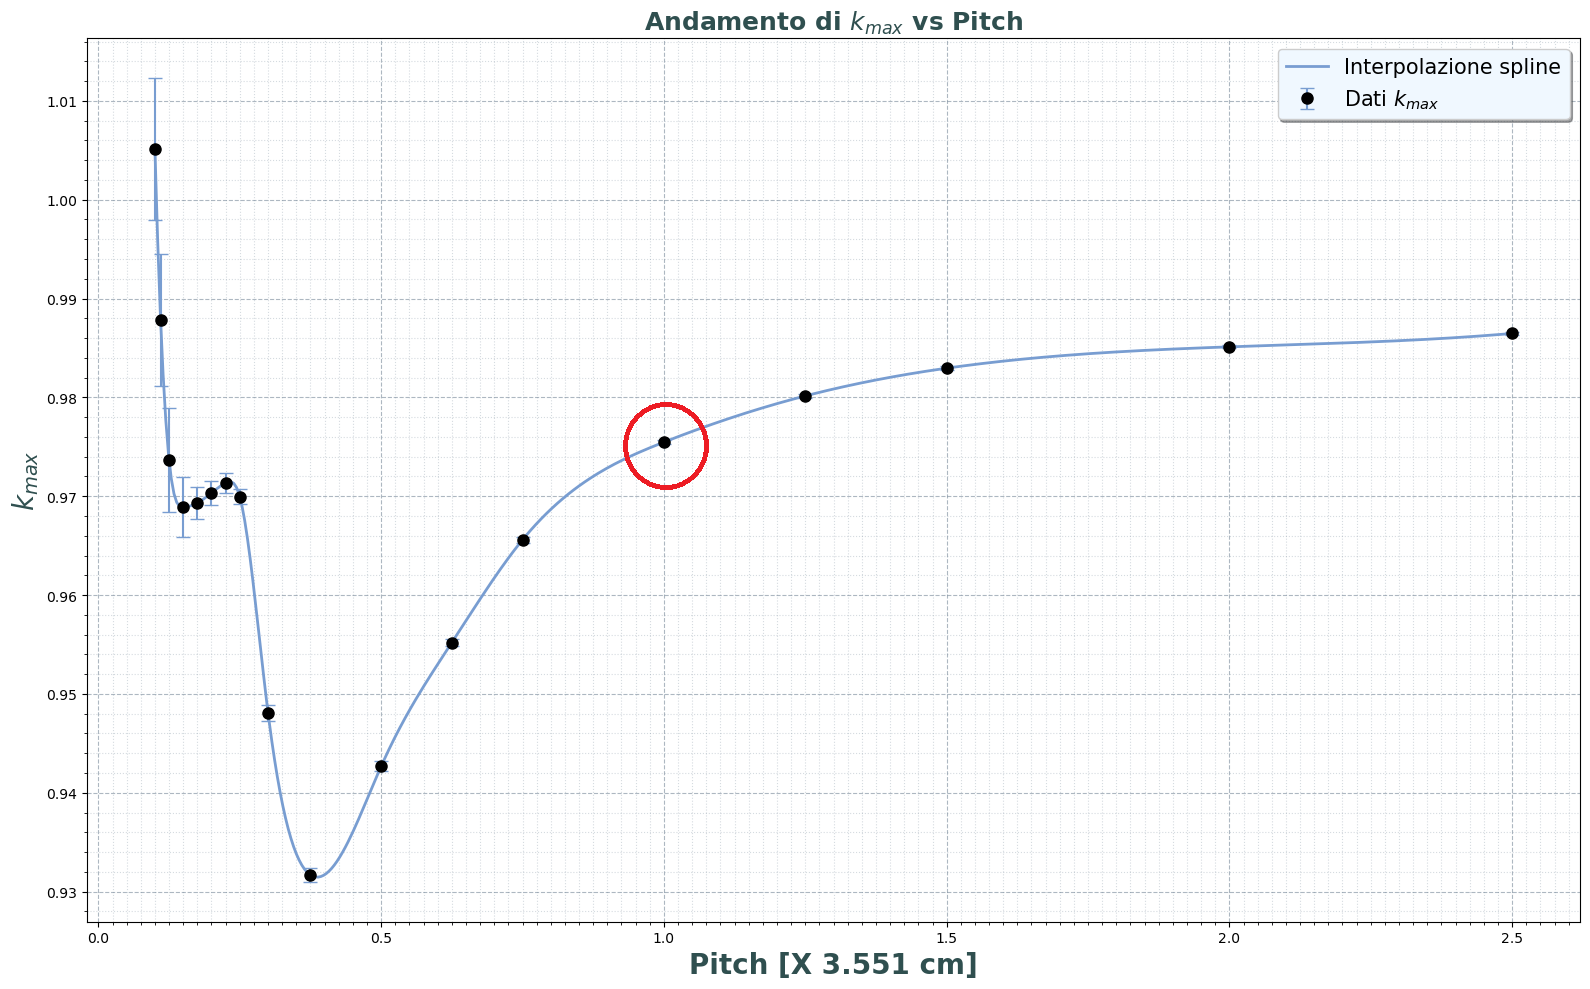
\includegraphics[width=0.65\textwidth]{pitch-k.png}
        \caption{ Modulazione di $k_{max}$ al variare esclusivo del Pitch del reticolo, evidenziando le zone di iper-moderazione e sotto-moderazione.}
        \label{fig:k_pitch}
    \end{figure}
\end{frame}

\begin{frame}{Topologia dell'Arricchimento}
    \begin{block}{Degenerazione Macroscopica}
        Dal punto di vista dell'autovalore fondamentale, fissato un pitch, il corrispondente $k_{max}$ è raggiungibile tramite molteplici combinazioni dell’arricchimento del core.
    \end{block}
    
    \vspace{0.3cm}
    \onslide<2->{
    \begin{alertblock}{Ridefinizione della geometria di arricchimento}
        Nel resto dei conti e simulazioni si è abbandonata la logica ad arricchimento omogeneo in favore di un \textbf{profilo lineare} tra l'anello di combustibile più interno e l'involucro esterno. 
    \end{alertblock}
    }
\end{frame}
\begin{frame}{Geometria ad Arricchiemnto variabile}
\begin{figure}
        \centering
      
        \begin{minipage}{0.48\textwidth}
            \centering
            
\includegraphics[width=0.9\linewidth]{reactor_xy_v.png}
            \caption{Sezione piano XY.}
        \end{minipage}
        \begin{minipage}{0.48\textwidth}
            \centering
            
\includegraphics[width=0.75\linewidth]{reactor_xz_v.png} % Larghezza ridotta per compensare l'altezza
            \caption{Sezione piano XZ.}
        \end{minipage}
    \end{figure}

    
\end{frame}

\begin{frame}{Spazio delle Soluzioni Stabili per un Pitch di 3.551 cm}
    \begin{figure}
        \centering
        
\includegraphics[width=0.78\textwidth]{regressione_parabolica_filtrata.png}
        \caption{ Locus dei punti di lavoro stabili}
        \label{fig:stabilità}
    \end{figure}
\end{frame}

\begin{frame}{Spazio delle Soluzioni Stabili}
    \begin{figure}
        \centering
        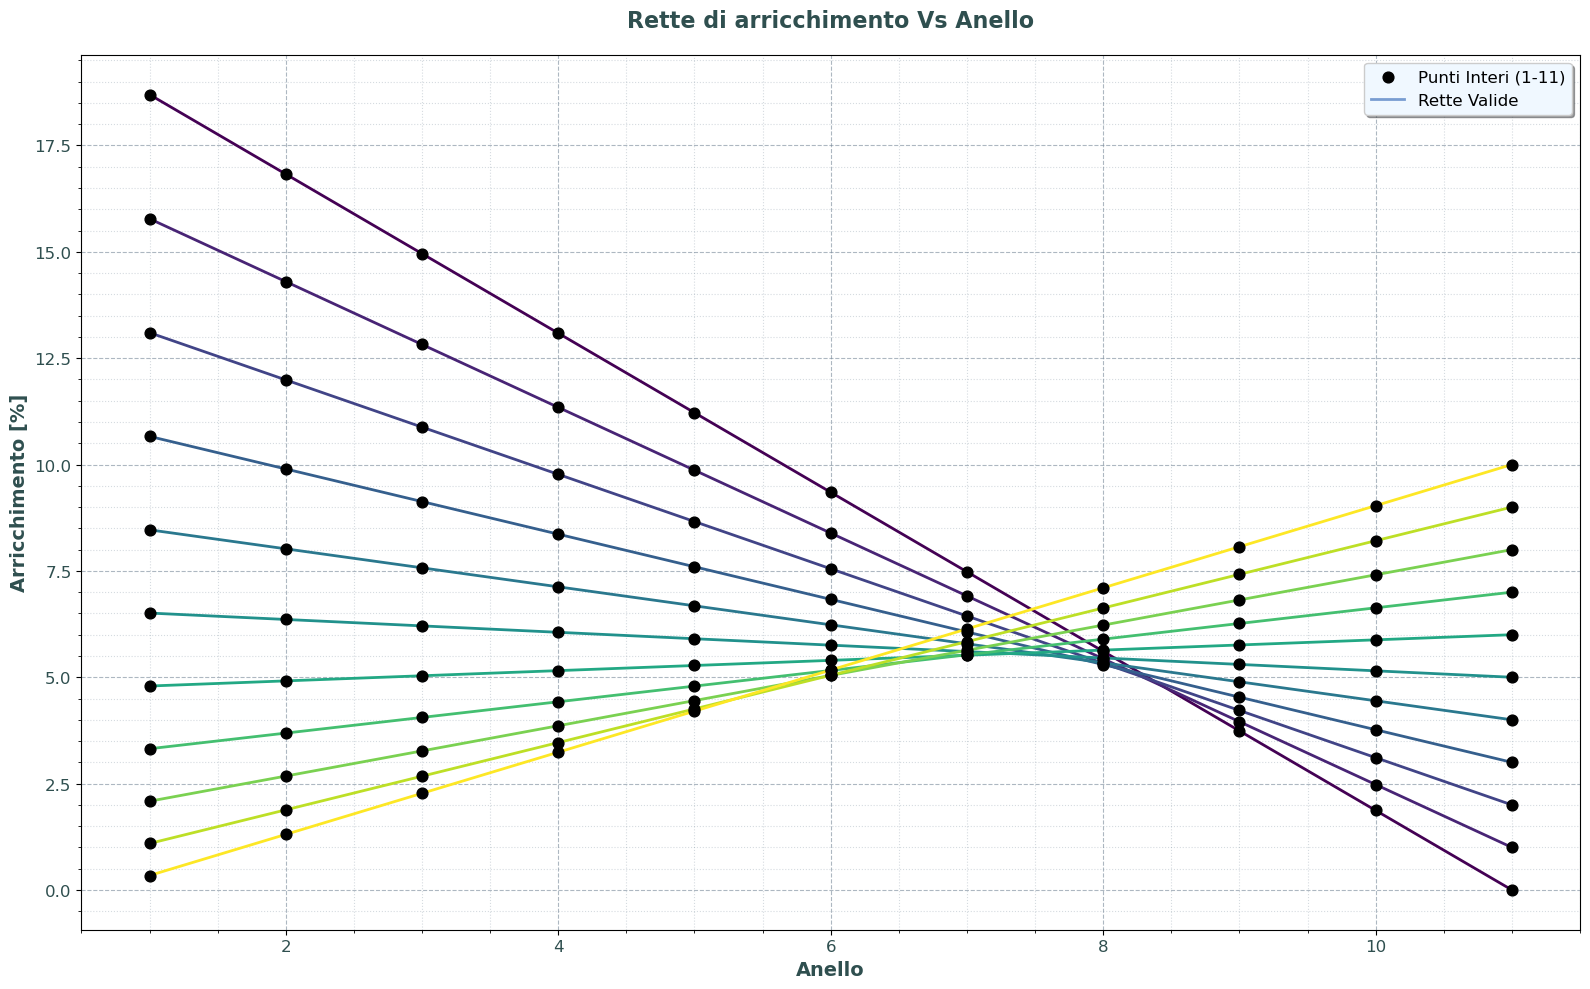
\includegraphics[width=0.68\textwidth]{rette_di_arricchimento.png}
        \caption{estrapolazione radiale per il gradiente di arricchimento.}
        \label{fig:stabilità2}
    \end{figure}
I punti di lavoro della slide precedente sono trovati con questa distribuzione radiale di arricchimenti
\end{frame}

\begin{frame}{Analisi in Sorgente Fissa}
    L'esecuzione in modalità sorgente fissa garantisce l'estrazione dei \textit{tally} di reattore esatti: spettro differenziale, distribuzioni spaziali di flusso, ratei di cattura e macro-fissioni, validando le dinamiche operative.
    
    \vspace{0.3cm}
    \onslide<2->{
    L'osservabile di primario interesse resta tuttavia la \textbf{Potenza Macroscopica}. Riportiamo qui i parametri inerenti il massimo di potenza ad un pitch x1, simulazione ad 1 Atm con arricchimento variabile linearmente : 
    
    \vspace{0.3cm}
    \begin{center}
        \setlength{\fboxsep}{12pt}
        \colorbox{blue!10}{
            \begin{tabular}{ll}
                \textbf{Fissioni per particella sorgente:} & 1.37078e-01 \\
                \textbf{Tasso di fissione reale:}       & 2.76897e+16 \text{ fissioni/s} \\
                \textbf{Potenza termica totale:}       &    0.887 MW\\
                \textbf{Q-factor (plasma physics):}        & 2.218
            \end{tabular}
        }
    \end{center}
    }
\end{frame}


\begin{frame}{Variazione della Potenza Estratta}
    \begin{figure}
        \centering
        
\includegraphics[width=0.7\textwidth]{scatter_potenza_errore.png}
        \caption{ Sensibilità della potenza termica macroscopica in funzione del grado di arricchimento radiale all'anello esterno}
        \label{fig:potenze}
    \end{figure}
\end{frame}


\begin{frame}{Parametri Prestazionali: Il Q-Factor}
    
    In un sistema ADS, il fattore di guadagno energetico $Q$ descrive l'amplificazione della potenza della sorgente nel nocciolo sottocritico:
    \begin{equation*}
        Q = \frac{P_{thermal}}{P_{beam}} = \psi \frac{k_{eff}}{1 - k_{eff}}
    \end{equation*}
    Dove $\psi$ rappresenta il fattore di importanza relativa dei neutroni di sorgente.
    
    Per una valutazione coerente si definisce un $Q_{sys}$ riferito alla potenza elettrica del sincrotrone:
    \begin{equation*}
        Q_{sys} = \frac{P_{thermal}}{P_{el, sync} / \eta_{th}} \approx 2.22
    \end{equation*}

    \begin{table}
        \centering
        \small
        \begin{tabular}{l | c | l}
            \textbf{Tecnologia} & \textbf{Q-Value (Target/Record)} & \textbf{Regime} \\
            \hline
            \textbf{ITER} & $\sim 10$ & Fusione (In costruzione) \\
            \textbf{SPARC} & $> 11$ & Fusione (In sviluppo) \\
            \textbf{JET} & $0.67$ & Fusione (Record 1997) \\
        \end{tabular}
    \end{table}
\end{frame}


\begin{frame}{Consistenza del Modello e Verifica di $k_{max}$}
    \begin{columns}[c]
        \begin{column}{0.5\textwidth}
            \begin{itemize}
                \item Validazione su diverse configurazioni di arricchimento lineare finalizzate all'uguaglianza con il $k_{max}$ di riferimento.
                \item Simulazioni eseguite sui tre stati termodinamici fondamentali: \textbf{CZP, HZP e HFP}.
                \item L'analisi della media pesata conferma la sostanziale invarianza dei valori di $k_{max}$ rispetto al caso limite ad arricchimento omogeneo.
                \item Questo comportamento convalida formalmente la flessibilità della metodologia geometrica adottata.
            \end{itemize}
        \end{column}
        
        \begin{column}{0.5\textwidth}
            \begin{figure}
                \centering
                % Inserire qui l'immagine: Andamento di k_max vs Arricchimento anello interno + confronti
                
\includegraphics[width=\linewidth]{circolarità.png}
            \end{figure}
        \end{column}
    \end{columns}
\end{frame}

\begin{frame}{Andamento di $k_{max}$ e Zone di Operatività}
    \begin{columns}[c]
        \begin{column}{0.5\textwidth}
            \begin{itemize}
                \item \textbf{Regione Verde (Operatività):} Dominio del pitch in cui è analiticamente possibile far convergere il sistema al $k_{max}$ target tramite modulazione dell'arricchimento.
                \item \textbf{Regione Rossa (Non Operatività):} Dominio inaccessibile. La corrispondenza con il $k_{max}$ fallisce anche imponendo un limite teorico di arricchimento omogeneo del $100\%$.
                \item \textbf{Dinamica Fisica:} La marcata non-linearità della funzione $k_{max}(\text{pitch})$ è governata dal bilancio di moderazione neutronica indotto dalla miscela di acqua leggera e pesante ($15\%$).
            \end{itemize}
        \end{column}
        
        \begin{column}{0.5\textwidth}
            \begin{figure}
                \centering
                % Inserire qui l'immagine: Andamento di k_max con evidenza delle zone di operatività
                
\includegraphics[width=\linewidth]{operatività.png}
            \end{figure}
        \end{column}
    \end{columns}
\end{frame}

% --- SLIDE 1: ANALISI DETTAGLIATA E FISICA DEL SISTEMA ---
\begin{frame}{Analisi della Risposta Termica e Ottimizzazione del Pitch}
    La caratterizzazione del reattore richiede la valutazione del legame tra parametri geometrici e prestazioni di potenza:

    \vspace{0.3cm}
    \begin{itemize}
        \item Esecuzione di una vasta campagna di simulazioni in regime \textit{fixed source} esclusivamente all'interno del dominio di operatività (Zona Verde), garantendo la stabilità neutronica del sistema.
        \item  L'andamento della potenza termica estrattibile è strettamente legato all'efficienza di rallentamento dei neutroni, determinata dal rapporto volumetrico tra moderatore ($15\%$ $D_2O$ in $H_2O$) e combustibile al variare del Pitch.
        \item  La competizione tra il rateo di fissione indotta e le perdite per fuga/cattura parassita determina un profilo di potenza non lineare.
        \item Attraverso un'interpolazione parabolica dei dati di simulazione, è stato individuato un punto di massimo globale per la potenza a un pitch equivalente di circa $14 \text{ cm}$.
    \end{itemize}
\end{frame}

% --- SLIDE 2: VISUALIZZAZIONE RISULTATI (LARGE IMAGE) ---
\begin{frame}{Analisi Accoppiata: Potenza e Moltiplicazione vs Pitch}
    \begin{figure}
        \centering
        % L'altezza è impostata per occupare quasi tutto lo spazio utile lasciando posto alla didascalia
        
\includegraphics[width=\linewidth]{potenza_kmax_vs_pitch.png}
        
        \vspace{0.2cm}
        \caption{\small Caratterizzazione delle prestazioni del core: correlazione tra il fattore di moltiplicazione $k_{max}$ e la potenza termica macroscopica generata in funzione del pitch reticolare. La curva di fit evidenzia l'ottimo di moderazione per il sistema ADS analizzato.}
    \end{figure}
\end{frame}

\begin{frame}{Next steps}
    \begin{itemize}
        \item Ulteriori test del modello con diversi pitch.
        \item Analisi di possibili altri meccanismi di feedback come per esempio i veleni.
        \item Analisi di sensibilità del modello con diverse geometrie e condizioni operative di pressione e moderatore.
    \end{itemize}
\end{frame}

\begin{frame}{}
    
\end{frame}

% --- SLIDE 1: Formulazione e Operatori ---
\begin{frame}{Fondamento Matematico: L'Equazione del Trasporto}
Il bilancio neutronico stazionario è governato dall'equazione del trasporto:

\begin{alertblock}{Formulazione Operatoriale}
\begin{equation*}
\mathcal{M} \Phi(\vec{r}, E, \hat{\Omega}) = \frac{1}{k_{eff}} \mathcal{F} \Phi(\vec{r}, E, \hat{\Omega})
 \end{equation*}
\end{alertblock}

I due operatori descrivono i ratei fisici in competizione nel nocciolo:

\begin{itemize}
\item \textbf{$\mathcal{M}$ (Operatore di Migrazione/Distruzione):} Quantifica le perdite nette. Include le fughe geometriche (\textit{streaming}, $\hat{\Omega} \cdot \nabla \Phi$), le interazioni totali ($\Sigma_t \Phi$) e i ripopolamenti cinematici dovuti allo scattering (\textit{in-scattering}).
\item \textbf{$\mathcal{F}$ (Operatore di Produzione):} Quantifica la sorgente stazionaria, descrivendo l'emissione di nuovi neutroni rapidi indotta dal rateo di fissione integrale ($\chi \nu \Sigma_f \Phi$).
\end{itemize}
\end{frame}

% --- SLIDE 2: Spettro e Significato Fisico ---
\begin{frame}{Fondamento Matematico: Il Teorema di Krein-Rutman}
Riscrivendo l'equazione come $\mathcal{M}^{-1}\mathcal{F} \Phi = k_{eff} \Phi$, l'operatore $\mathcal{M}^{-1}\mathcal{F}$ mappa una generazione di neutroni in quella successiva. Essendo le densità atomiche e le sezioni d'urto quantità strettamente positive, tale operatore è \textbf{rigorosamente positivo}.

\begin{block}{Dominanza dell'Autovalore ($k_{eff}$)}
Per il \textbf{Teorema di Krein-Rutman}, un operatore integrale positivo garantisce l'esistenza di un autovalore fondamentale ($k_0 \equiv k_{eff}$) reale, positivo e \textbf{maggiore in modulo} di tutti gli altri autovalori dello spettro ($|k_0| > |k_n|$).
\end{block}

\begin{alertblock}{Significato Fisico dell'Autofunzione ($\Phi_0$)}
Solo all'autovalore dominante $k_{eff}$ è associata un'autofunzione $\Phi_0$ \textbf{ovunque definita positiva}. Le armoniche di ordine superiore presentano inevitabilmente dei nodi (flussi negativi, fisicamente impossibili in stazionario).
\end{alertblock}
\end{frame}


\end{document}